\documentclass[12pt]{article}
\usepackage[margin=1in]{geometry}
\usepackage{setspace}
\usepackage[T1]{fontenc}
\usepackage{newtxtext,newtxmath}
\usepackage{graphicx}
\usepackage{float}
\usepackage{booktabs}
\usepackage{tabularx}
\usepackage{array}
\usepackage{ragged2e}
\usepackage{caption}
\usepackage[table]{xcolor}
\usepackage{hyperref}
\usepackage{colortbl}
\usepackage{hhline}

\doublespacing
\setlength{\parindent}{0pt}
\setlength{\parskip}{0.5em}
\setlength{\tabcolsep}{5.4pt}
\renewcommand{\arraystretch}{1.42}
\setlength{\extrarowheight}{1.5pt}
\setlength{\emergencystretch}{2em}
\captionsetup{font={small,stretch=1},labelfont=bf}
\setlength{\arrayrulewidth}{1.0pt}
\arrayrulecolor{black}

\definecolor{stagecollect}{HTML}{365C8D}
\definecolor{stageclean}{HTML}{2E7D6E}
\definecolor{stageprep}{HTML}{C97A2B}
\definecolor{stagemine}{HTML}{7B4FA0}
\definecolor{lightcollect}{HTML}{EAF1F8}
\definecolor{lightclean}{HTML}{E8F4F1}
\definecolor{lightprep}{HTML}{FBF1E4}
\definecolor{lightmine}{HTML}{F1E9F8}
\definecolor{tableheader}{HTML}{F2F2F2}

\newcolumntype{L}[1]{>{\RaggedRight\arraybackslash}p{#1}}
\newcolumntype{Y}{>{\RaggedRight\arraybackslash}X}

\newcommand{\HlineFive}{\hhline{|-----|}}
\newcommand{\HlineSeven}{\hhline{|-------|}}
\newcommand{\cellstack}[1]{\shortstack[l]{#1}}

\newcommand{\stagecell}[2]{\cellcolor{#1!14}\textcolor{#1}{\textbf{#2}}}
\newcommand{\metriccell}[2]{\cellcolor{#1!14}\textbf{#2}}
\DeclareRobustCommand{\artifact}[1]{\texttt{#1}}
\newcommand{\cmd}[1]{\texttt{\detokenize{#1}}}

\title{Materials and Methods Draft\\Mouse DRG RNA-seq Follow-up Project}
\author{Piter Garcia}
\date{Draft prepared for BIOL550}

\begin{document}
\maketitle

\section{Materials and Methods}

This project reanalyzed mouse DRG bulk RNA-seq after sciatic nerve injury using a four-stage workflow modeled after a CRISP-style progression: \textbf{Data Collection}, \textbf{Data Cleaning}, \textbf{Data Preparation}, and \textbf{Data Analysis and Interpretation}. That structure was not added only for presentation. It reflects how the \artifact{mouse\_new} workflow was built and refined across the weekly reports, where each stage owned a specific handoff, a checkpoint artifact, and a reusable output for the next stage. The same staged structure also made it possible to reuse the pipeline after earlier dataset-selection problems, because accession tracking, QC review, alignment review, and downstream modeling were separated into explicit, repeatable checkpoints instead of being handled as one monolithic notebook run.

The working subset comprised 20 NovaSeq X paired-end libraries from \artifact{SRP618841} (BioProject \artifact{PRJNA1017789}; GEO \artifact{GSE243308}), organized as a balanced side-by-genotype design before quality control, alignment, and differential expression modeling. In practice, the weekly reports served as the running record of how this dataset was narrowed, checked, and carried forward, while the final Methods draft translates that same path into manuscript prose.

\begin{figure}[H]
\centering
\makebox[\textwidth][c]{
\includegraphics[width=1.02\textwidth]{assets_methods/overview_pipeline_stage.png}}
\caption{Overview ribbon summarizing the four computational stages and their stage-owned handoffs in the \artifact{mouse\_new} workflow.}
\label{fig:overall_pipeline}
\end{figure}

\begin{table}[H]
\centering
\begin{singlespace}
\fontsize{7.0}{7.7}\selectfont
\caption{Pipeline checkpoint table used to anchor the Methods section to stage-specific evidence.}
\label{tab:pipeline_checkpoint}
\begin{tabularx}{\textwidth}{|Y|Y|Y|Y|Y|}
\HlineFive
\rowcolor{tableheader}
\textbf{Stage} & \textbf{Primary artifacts} & \textbf{Core tools} & \textbf{Checkpoint metric} & \textbf{Handoff} \\
\HlineFive
\stagecell{stagecollect}{Collection} &
sample table; family sheet &
\artifact{prefetch} + \artifact{fasterq-dump} &
\metriccell{stagecollect}{20 SRRs retained; 4 balanced subgroups ($n=5$ each)} &
\artifact{FASTQ.gz} pairs + manifest \\
\HlineFive

\stagecell{stageclean}{Cleaning} &
QC heatmap; severity delta &
\artifact{FastQC} + \artifact{MultiQC} + \artifact{fastp} &
\metriccell{stageclean}{raw adapter-content failures resolved after trimming} &
trimmed read pairs plus per-sample QC reports \\
\HlineFive

\stagecell{stageprep}{Preparation} &
unique-mapping plot; STAR median summary &
\artifact{STAR} + \artifact{GeneCounts} &
\metriccell{stageprep}{93.24\% median unique mapping; 3.82\% median \artifact{noFeature}} &
sorted BAMs, STAR logs, count tables, and family matrix \\
\HlineFive

\stagecell{stagemine}{Analysis} &
\cellstack{filtering summary\\analysis summary\\g:Profiler source tables} &
\artifact{DESeq2} + bend-point + \artifact{g:Profiler} &
\metriccell{stagemine}{78{,}334 $\rightarrow$ 21{,}481 genes after filtering; 5 modeled contrasts} &
DE tables, bend-point follow-up sets, and enrichment summaries \\
\HlineFive
\end{tabularx}
\end{singlespace}
\end{table}

\subsection{Representative command examples}
The course draft requirements asked for sample commands for each major tool. Table~\ref{tab:command_examples} therefore provides short representative examples showing how the main workflow stages were executed. These examples are included to document the computational path and major non-default parameters; they are illustrative rather than exhaustive wrapper scripts.

\begin{table}[H]
\centering
\begin{singlespace}
\fontsize{6.6}{7.2}\selectfont
\caption{Representative command examples for the tools used in the \artifact{mouse\_new} workflow.}
\label{tab:command_examples}
\begin{tabularx}{\textwidth}{|L{0.16\textwidth}|L{0.20\textwidth}|Y|}
\hline
\rowcolor{tableheader}
\textbf{Stage} & \textbf{Tool} & \textbf{Representative command / code example} \\
\hline
\stagecell{stagecollect}{Collection} & \cellstack{\artifact{prefetch}\\\artifact{fasterq-dump}} & \cmd{prefetch SRRXXXXXXX && fasterq-dump SRRXXXXXXX --split-files -O fastq/} \\
\hline
\stagecell{stageclean}{Cleaning} & \artifact{FastQC} & \cmd{fastqc raw/*.fastq.gz trimmed/*.fastq.gz --outdir fastqc_reports/} \\
\hline
\stagecell{stageclean}{Cleaning} & \artifact{MultiQC} & \cmd{multiqc fastqc_reports/ fastp_reports_full/ -o multiqc/} \\
\hline
\stagecell{stageclean}{Cleaning} & \artifact{fastp} & \cellstack{\cmd{fastp -i sample_R1.fastq.gz -I sample_R2.fastq.gz}\\\cmd{-o clean_R1.fastq.gz -O clean_R2.fastq.gz}\\\cmd{--detect_adapter_for_pe --trim_poly_g}\\\cmd{--cut_mean_quality 20 --length_required 30}\\\cmd{-h sample.html -j sample.json}} \\
\hline
\stagecell{stageprep}{Preparation} & \artifact{STAR} & \cellstack{\cmd{STAR --runThreadN 8 --genomeDir star_index}\\\cmd{--readFilesIn clean_R1.fastq.gz clean_R2.fastq.gz}\\\cmd{--readFilesCommand zcat}\\\cmd{--sjdbGTFfile Mus_musculus.GRCm39.115.gtf}\\\cmd{--outSAMtype BAM SortedByCoordinate --quantMode GeneCounts}} \\
\hline
\stagecell{stagemine}{Analysis} & \artifact{DESeq2} & \cmd{dds <- DESeqDataSetFromMatrix(countData, colData, design = ~ side_class * geno_class); dds <- DESeq(dds)} \\
\hline
\stagecell{stagemine}{Analysis} & bend-point scripts & \cmd{python3 run_bendpoint_followup.py --contrast ipsi_vs_contra_in_ff --padj-column padj} \\
\hline
\stagecell{stagemine}{Analysis} & \artifact{g:Profiler} & \cmd{gp.profile(organism = "mmusculus", query = selected_genes, sources = c("GO:BP","KEGG","REAC"))} \\
\hline
\end{tabularx}
\end{singlespace}
\end{table}

\subsection{Data Collection: SRA Acquisition and Sample Organization}
The analysis began with the published DRG RNA-seq study \artifact{SRP618841}, linked to BioProject \artifact{PRJNA1017789} and GEO series \artifact{GSE243308}. Public runs were retrieved using the project wrappers around \artifact{prefetch} and \artifact{fasterq-dump}, and the local workflow retained 20 paired-end NovaSeq X libraries from the 1-day-post-injury DRG subset. Recording this accession lineage was important because the pipeline had to remain reusable across candidate mouse datasets; explicit accession-to-run tracking prevented later stages from being tied to an ambiguous ``mouse'' source.

After download, metadata were consolidated into a design-aware sample table rather than being left as file-name strings. Each retained sample was annotated by \artifact{side\_class} (\artifact{ipsi} or \artifact{contra}), \artifact{geno\_class} (\artifact{ff} or \artifact{cre}), and the derived \artifact{condition\_family}. This step established the balanced 2$\times$2 design used in the DESeq2 model and in subsequent interpretation. It also created a reusable family manifest that could be re-read by downstream notebooks and figure builders without having to reconstruct group identity from filenames each time.

\begin{figure}[H]
\centering
\makebox[\textwidth][c]{
\includegraphics[width=1.02\textwidth]{assets_methods/data_collection_stage.png}}
\caption{Rebuilt Data Collection stage figure derived from the saved project metadata and design tables.}
\label{fig:data_collection}
\end{figure}

\begin{table}[H]
\centering
\begin{singlespace}
\fontsize{7.2}{8.1}\selectfont
\caption{Data Collection stage table.}
\label{tab:data_collection}
\begin{tabularx}{\textwidth}{|Y|Y|Y|Y|Y|}
\HlineFive
\rowcolor{tableheader}
\textbf{Substage} & \textbf{Input} & \textbf{Tool} & \textbf{Checkpoint artifact / evidence} & \textbf{Why it mattered} \\
\HlineFive
\stagecell{stagecollect}{Study provenance} &
public accession records &
SRA / GEO review &
accession lineage shown in Figure~\ref{fig:data_collection}: \artifact{SRP618841} $\rightarrow$ \artifact{PRJNA1017789} $\rightarrow$ \artifact{GSE243308} &
anchors the Methods section to the exact source study \\
\HlineFive

\stagecell{stagecollect}{Run acquisition} &
public SRA runs &
\cellstack{\artifact{prefetch}\\\artifact{fasterq-dump}} &
paired-end \artifact{FASTQ.gz} files plus the local run manifest; 20 retained SRRs from the DRG / NovaSeq X subset &
creates the fixed read set used throughout the pipeline \\
\HlineFive

\stagecell{stagecollect}{Design mapping} &
run manifest + sample titles &
local manifest assembly &
design table and family sample sheet; 5 samples in each subgroup &
makes the side/genotype structure explicit before PCA and DE modeling \\
\HlineFive
\end{tabularx}
\end{singlespace}
\end{table}

\subsection{Data Cleaning: Quality Control and Read Trimming}
Raw read quality was evaluated with \artifact{FastQC}, and cohort-level summaries were consolidated with \artifact{MultiQC}. This stage was treated as a documented checkpoint rather than a minimal preprocessing step, so before-and-after QC artifacts were retained to show the effect of trimming explicitly. The local workflow used \artifact{fastp} v0.23.2 as the canonical cleanup tool because it provided a reproducible paired-end workflow, generated per-sample reports that could be reviewed later, and resolved adapter-related signal more effectively than the earlier baseline.

The retained \artifact{fastp} configuration used paired-end adapter detection, poly-G trimming, a mean-quality cutoff of 20, a minimum retained length of 30 bases, and per-sample HTML/JSON reporting. In Figure~\ref{fig:data_cleaning}, the left panel shows the module-status heatmap and the right panel shows the SRR-level severity-change plot. Together, these artifacts document a consistent improvement in read quality across the cohort before alignment. Keeping both the raw and trimmed checkpoints made this stage reusable for later dataset screening, because poor candidate subsets could be rejected or repaired using the same evidence trail rather than by ad hoc trimming decisions.

\begin{figure}[H]
\centering
\makebox[\textwidth][c]{
\includegraphics[width=1.04\textwidth]{assets_methods/data_cleaning_stage.png}}
\caption{Data Cleaning stage figure using retained QC artifacts and a rebuilt checkpoint strip.}
\label{fig:data_cleaning}
\end{figure}

\begin{table}[H]
\centering
\begin{singlespace}
\fontsize{7.2}{8.1}\selectfont
\caption{Data Cleaning stage table.}
\label{tab:data_cleaning}
\fontsize{6.9}{7.8}\selectfont
\begin{tabularx}{\textwidth}{|Y|Y|Y|Y|Y|}
\HlineFive
\rowcolor{tableheader}
\textbf{Substage} & \textbf{Input} & \textbf{Tool} & \textbf{Checkpoint artifact / evidence} & \textbf{Why it mattered} \\
\HlineFive
\stagecell{stageclean}{Raw QC} &
raw paired-end reads &
\artifact{FastQC} + \artifact{MultiQC} &
raw module-status heatmap and cohort QC summary; adapter-content failures across all 40 raw read files &
establishes the baseline quality state before trimming \\
\HlineFive

\stagecell{stageclean}{Read trimming} &
raw \artifact{FASTQ.gz} pairs &
\artifact{fastp} v0.23.2 &
\cellstack{trimmed read pairs\\per-sample HTML/JSON reports; PE adapter detect,\\Q20 cutoff, min length 30 bp,\\poly-G trimming} &
standardizes cleanup across all retained libraries \\
\HlineFive

\stagecell{stageclean}{Post-trim checkpoint} &
trimmed read pairs &
\artifact{FastQC} + \artifact{MultiQC} &
saved SRR-level severity summary; all retained severity deltas moved in the negative direction after trimming &
justifies using the cleaned reads, not the raw reads, for alignment \\
\HlineFive
\end{tabularx}
\end{singlespace}
\end{table}

\subsection{Data Preparation: Reference Selection and Alignment}
Trimmed read pairs were aligned to the \textit{Mus musculus} \artifact{GRCm39} primary assembly with the matching Ensembl release 115 annotation. The reference pair used in the local workflow consisted of \artifact{Mus\_musculus.GRCm39.dna.primary\_assembly.fa} and \artifact{Mus\_musculus.GRCm39.115.gtf}. A STAR genome index was generated with \artifact{sjdbOverhang = 150} to match the 151-bp paired-end reads. Alignment was performed with STAR using gzip-aware input handling, coordinate-sorted BAM output, and \artifact{GeneCounts} so that the same run also produced per-sample count tables.

This stage linked cleaned reads to downstream modeling through a stable alignment handoff. For each sample, the workflow retained three key outputs: a coordinate-sorted BAM file, a STAR \artifact{Log.final.out} summary, and a \artifact{ReadsPerGene.out.tab} count table. These outputs provided both the alignment checkpoint and the count-level handoff used to assemble the final family matrix for the DRG subset. Treating the alignment review and the count-matrix assembly as explicit handoffs made it possible to reuse the same preparation stage across datasets without rewriting the downstream DE workflow.

\begin{figure}[H]
\centering
\makebox[\textwidth][c]{
\includegraphics[width=1.04\textwidth]{assets_methods/data_preparation_stage.png}}
\caption{Data Preparation stage figure built from retained STAR outputs and rebuilt alignment checkpoint metrics.}
\label{fig:data_preparation}
\end{figure}

\begin{table}[H]
\centering
\begin{singlespace}
\fontsize{7.2}{8.1}\selectfont
\caption{Data Preparation stage table.}
\label{tab:data_preparation}
\begin{tabularx}{\textwidth}{|Y|Y|Y|Y|Y|}
\HlineFive
\rowcolor{tableheader}
\textbf{Substage} & \textbf{Input} & \textbf{Tool} & \textbf{Checkpoint artifact / evidence} & \textbf{Why it mattered} \\
\HlineFive
\stagecell{stageprep}{Reference choice} &
mouse genome + annotation &
Ensembl reference selection &
reference FASTA/GTF pair for \artifact{GRCm39} primary assembly + Ensembl v115 annotation &
locks the coordinate system used by STAR and downstream counts \\
\HlineFive

\stagecell{stageprep}{STAR index \& run} &
trimmed read pairs + reference &
\artifact{STAR} &
sorted BAM, \artifact{Log.final.out}, and \artifact{ReadsPerGene.out.tab}; \artifact{sjdbOverhang = 150} and paired-end alignment/counting in one run &
produces the alignment checkpoint and the count-ready artifacts in one run \\
\HlineFive

\stagecell{stageprep}{Alignment checkpoint} &
saved STAR summaries &
local alignment review &
retained unique-mapping plot plus the STAR median summary table; unique 93.24\%, multi 5.10\%, \artifact{noFeature} 3.82\%, ambiguous 1.77\% &
confirms the cleaned reads mapped well enough to move into DESeq2 \\
\HlineFive

\stagecell{stageprep}{Count handoff} &
per-sample count outputs &
local merge scripts / notebooks &
family-level count matrix for \artifact{family\_drg\_novaseqx}; 20 samples retained in the final family matrix &
converts per-sample STAR outputs into the DE-ready family matrix \\
\HlineFive
\end{tabularx}
\end{singlespace}
\end{table}

\subsection{Data Analysis and Interpretation: Differential Expression and Functional Analysis}
The merged family count matrix was analyzed with \artifact{DESeq2} using the explicit side-by-genotype design carried forward from the sample manifest. Before modeling, low-support genes were filtered, reducing the tested set from 78{,}334 genes to 21{,}481 while retaining all 20 DRG samples. Five contrasts were then evaluated: \artifact{ipsi\_vs\_contra\_in\_ff}, \artifact{ipsi\_vs\_contra\_in\_cre}, \artifact{geno\_in\_contra}, \artifact{geno\_in\_ipsi}, and \artifact{interaction}. This contrast inventory was kept fixed so that later interpretation did not drift when one branch became more interpretable than another.

As documented in the weekly reports, downstream interpretation followed a PCA-first and branch-priority logic rather than a raw gene-count logic. PCA was used to read sample structure before long DE tables were emphasized, and the side-specific branches were then carried forward as the primary follow-up path. To avoid reducing very large DE outputs to unstructured gene lists, the workflow applied a bend-point rule to the ordered adjusted-\textit{p}-value curve for each contrast. These bend-point-derived follow-up sets were therefore reported alongside the \artifact{padj < 0.05} results rather than treated as interchangeable with them. For the two primary side-specific contrasts, this step retained 709 and 870 genes, respectively.

The resulting follow-up sets were then submitted to \artifact{g:Profiler} using GO Biological Process, KEGG, and Reactome layers. In the \artifact{ff} branch, which remained the clearest pathway-level follow-up in the weekly reports, enrichment outputs were later re-read through shared-gene chart, tree, and network views to reduce redundancy among overlapping GO labels. In this Methods framing, those enrichment products are described as reusable downstream summaries of the DE workflow rather than as final biological claims.

\begin{figure}[H]
\centering
\makebox[\textwidth][c]{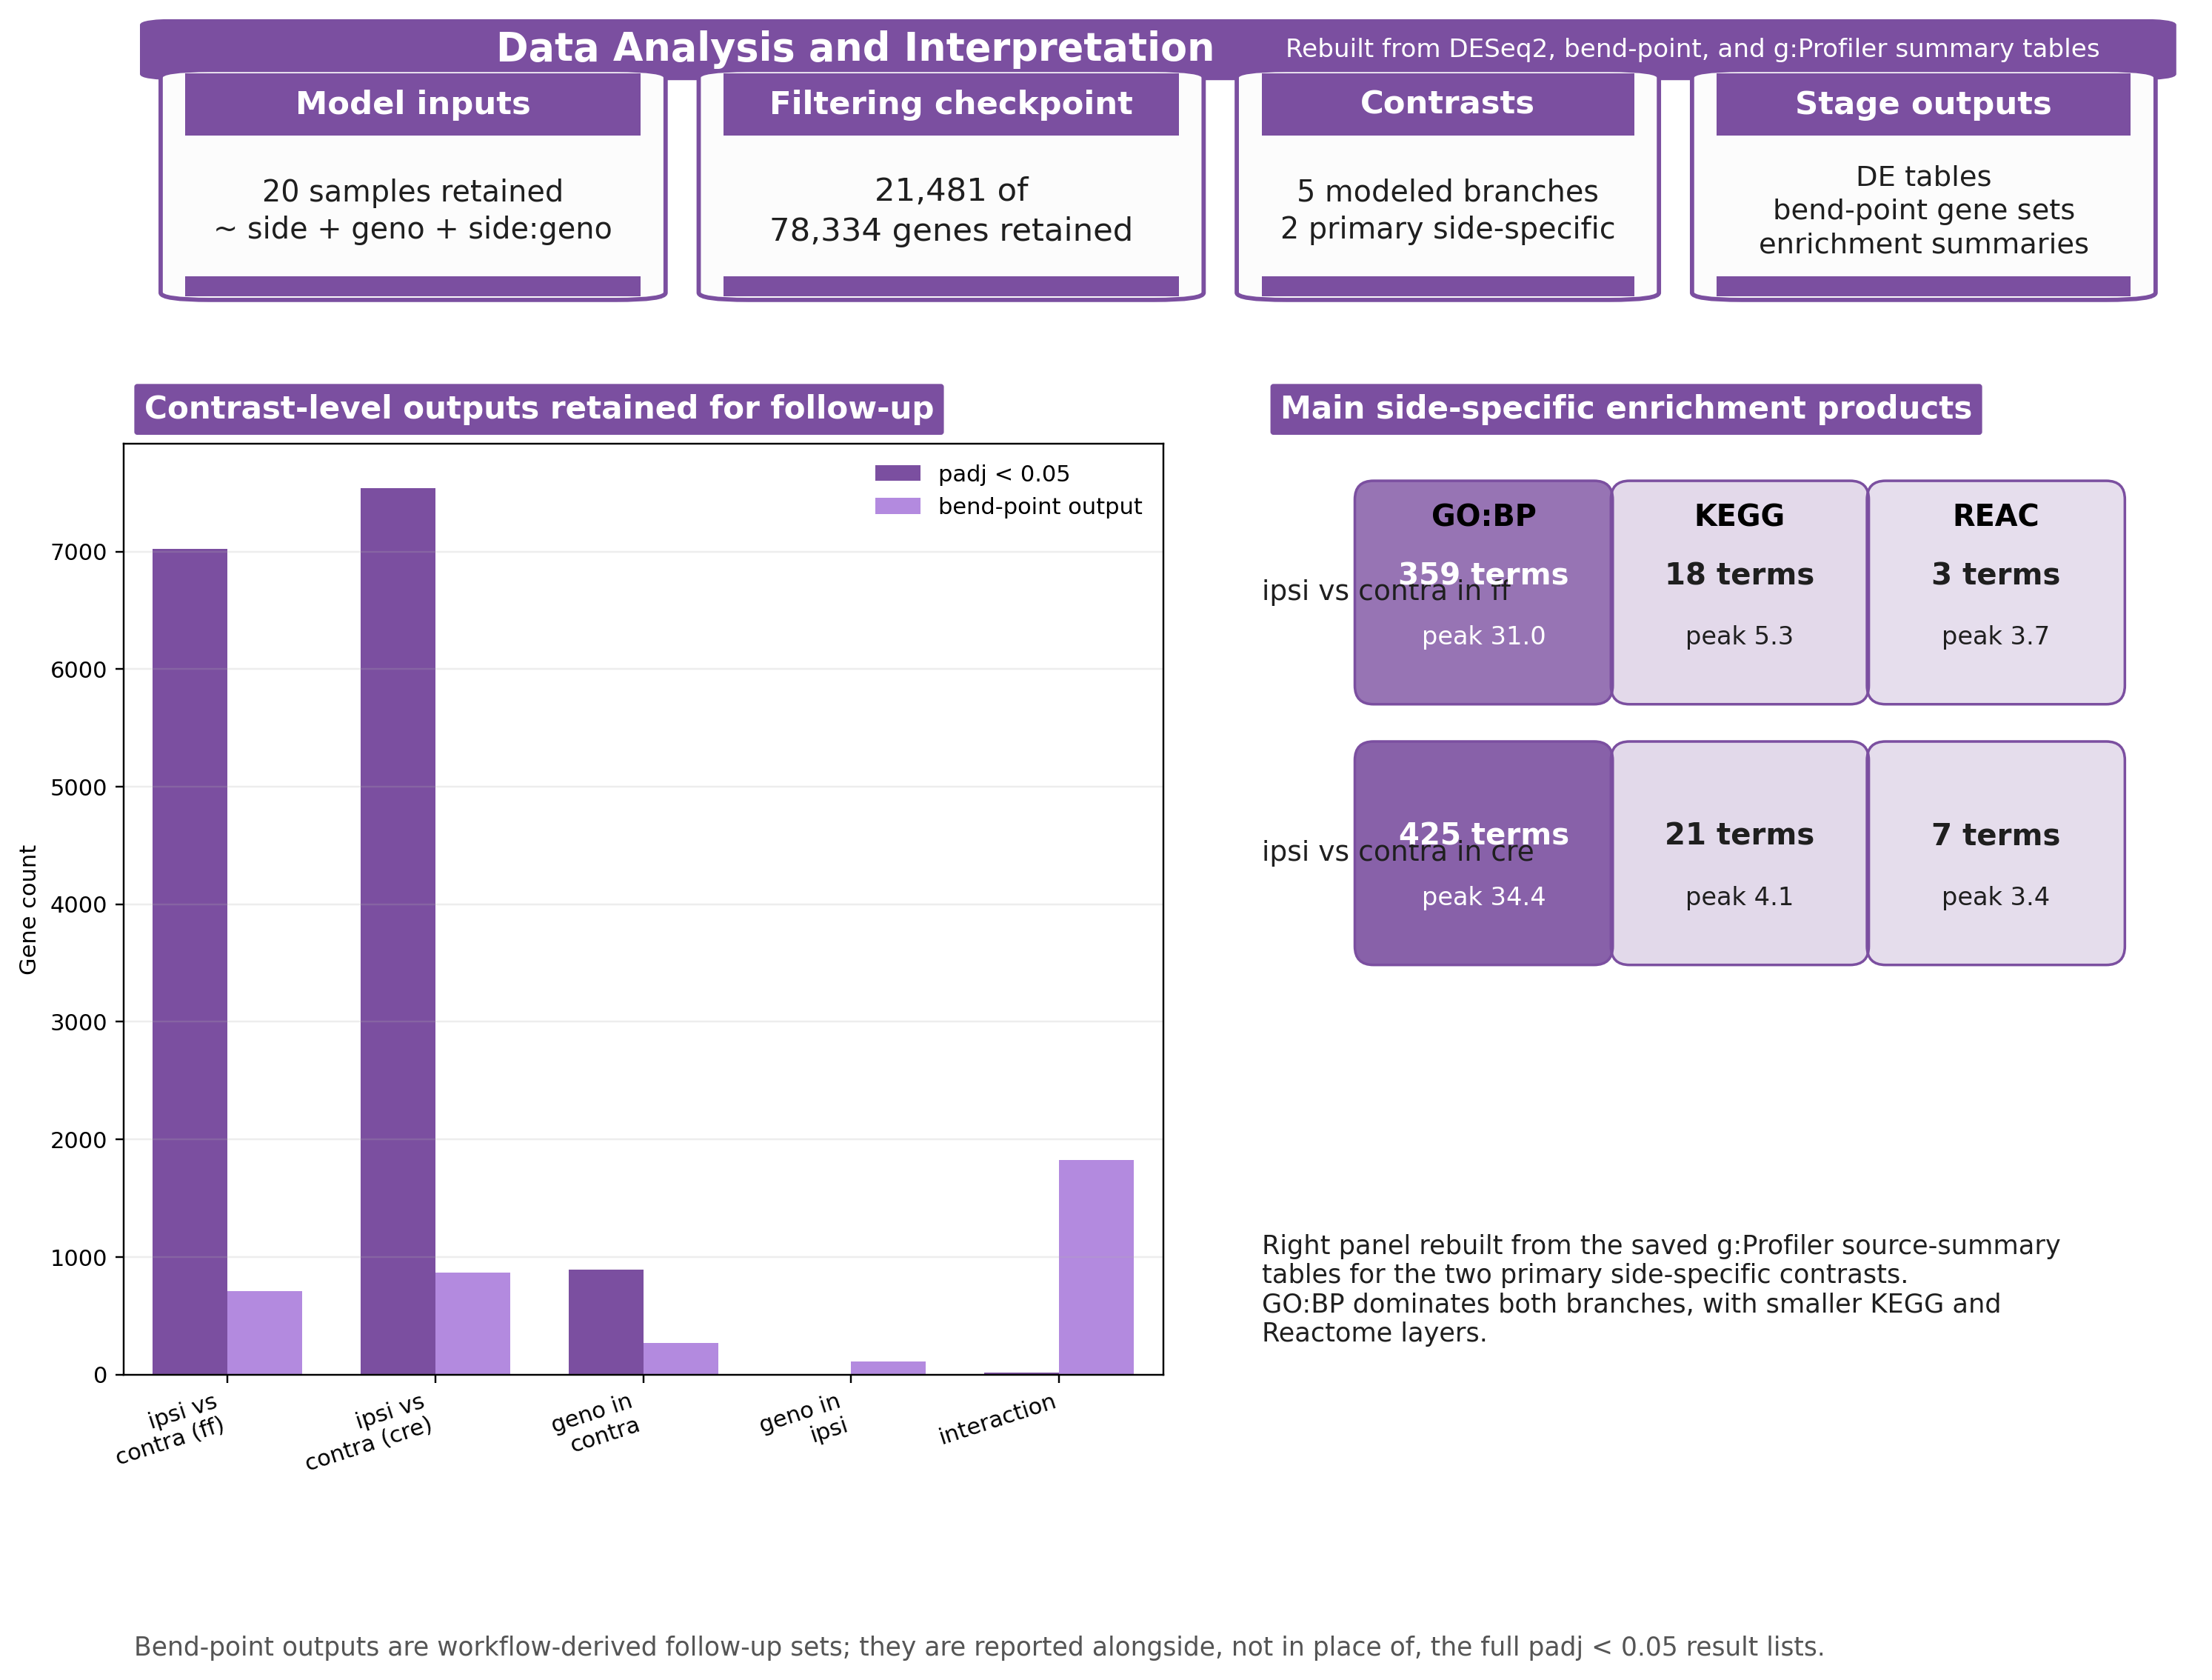
\includegraphics[width=1.04\textwidth]{assets_methods/data_mining_stage.png}}
\caption{Rebuilt Data Analysis and Interpretation stage figure derived from saved \artifact{DESeq2}, bend-point, and \artifact{g:Profiler} summary tables.}
\label{fig:data_analysis}
\end{figure}

\begin{figure}[H]
\centering
\makebox[\textwidth][c]{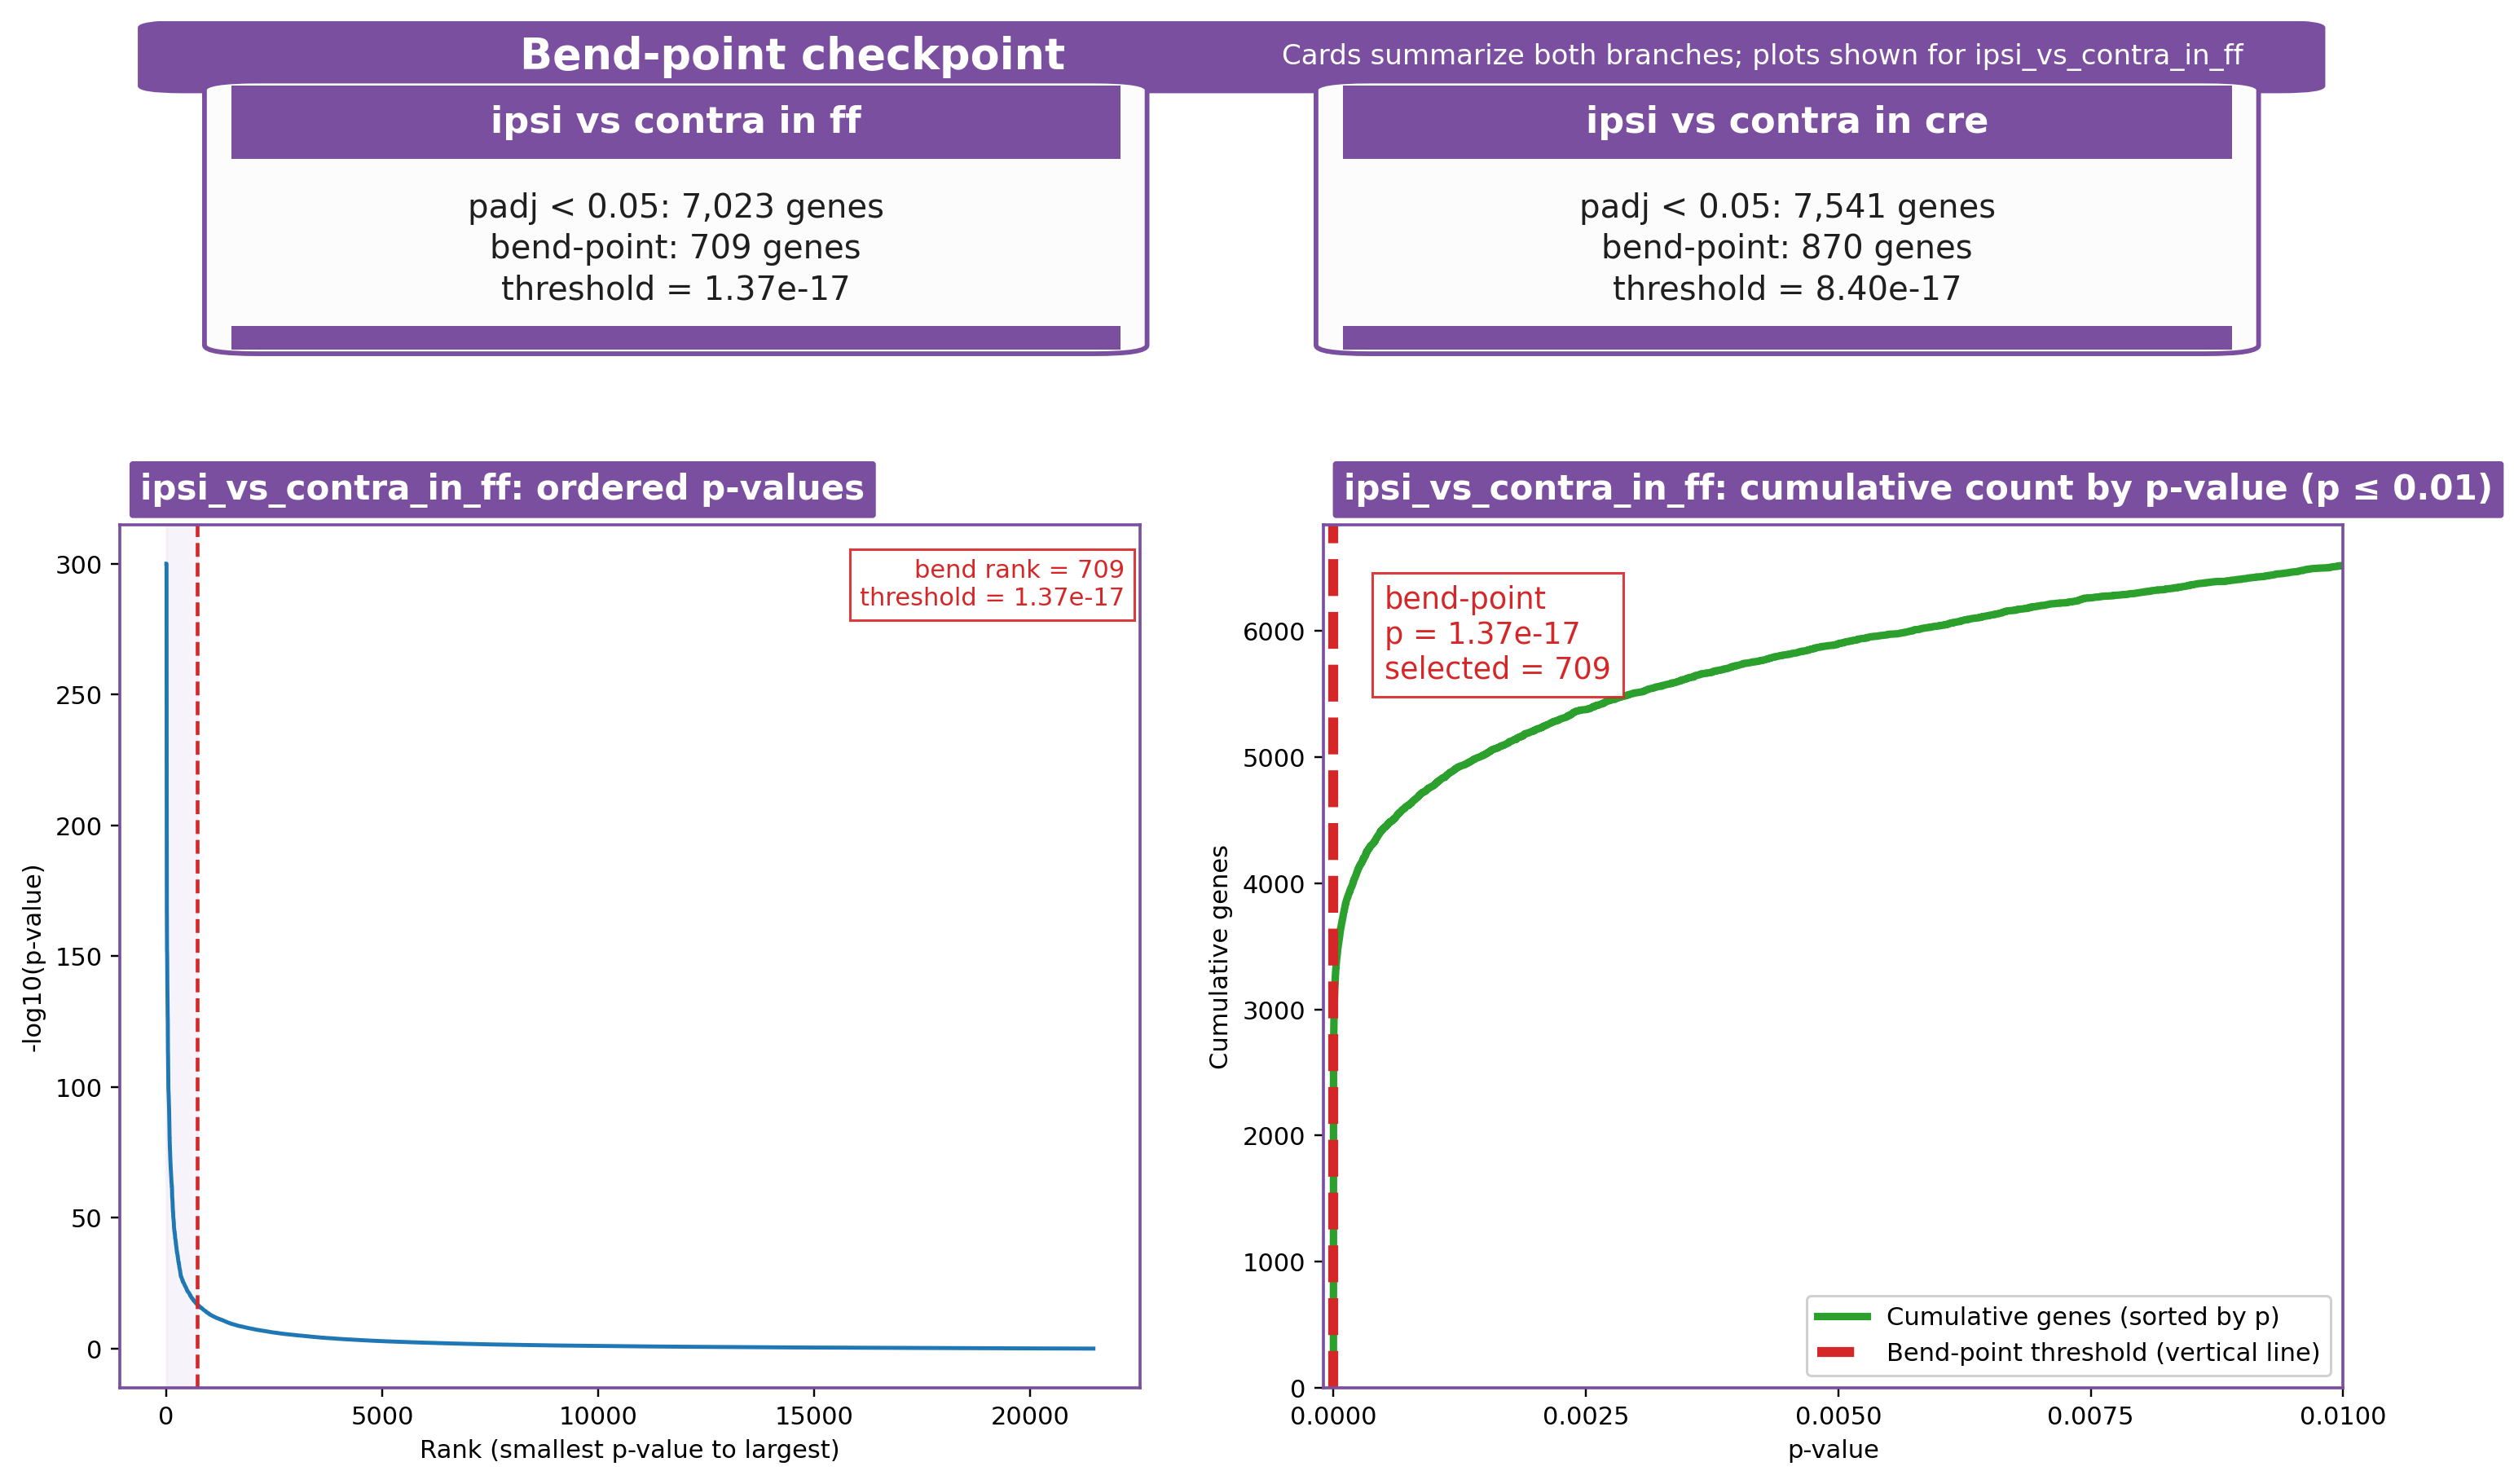
\includegraphics[width=1.04\textwidth]{assets_methods/data_mining_selection_stage.png}}
\caption{Retained bend-point checkpoint summary for the two primary side-specific branches (cards). The ordered p-value and cumulative-count plots are shown for the \artifact{ipsi\_vs\_contra\_in\_ff} example, with the right panel zoomed to \textit{p} $\le$ 0.01.}
\label{fig:data_analysis_selection}
\end{figure}

\begin{table}[H]
\centering
\begin{singlespace}
\fontsize{7.1}{8.0}\selectfont
\caption{Data Analysis and Interpretation workflow table.}
\label{tab:data_analysis}
\begin{tabularx}{\textwidth}{|Y|Y|Y|Y|Y|}
\HlineFive
\rowcolor{tableheader}
\textbf{Substage} & \textbf{Input} & \textbf{Tool} & \textbf{Checkpoint artifact / evidence} & \textbf{Why it mattered} \\
\HlineFive
\stagecell{stagemine}{Model setup} &
family count matrix + design table &
\artifact{DESeq2} &
normalized counts, VST matrix, and contrast-level result tables; 20 samples retained and 78{,}334 $\rightarrow$ 21{,}481 genes after filtering &
defines the inferential base for every contrast and downstream plot \\
\HlineFive

\stagecell{stagemine}{Contrast production} &
filtered model outputs &
\cellstack{\artifact{DESeq2}\\contrast manifest} &
five saved contrast branches; two primary side-specific and three supporting genotype / interaction branches &
keeps the main and supporting stories explicit before list narrowing \\
\HlineFive

\stagecell{stagemine}{Bend-point selection} &
ordered adjusted-\textit{p} tables &
local bend-point scripts &
analysis-summary and per-contrast bend-point summary tables; primary side-specific follow-up sets of 709 genes in \artifact{ff} and 870 genes in \artifact{cre} &
turns very large DE lists into smaller reproducible follow-up sets \\
\HlineFive

\stagecell{stagemine}{Enrichment layer} &
bend-point-selected gene sets &
\artifact{g:Profiler} &
g:Profiler source-summary and enrichment tables; the main \artifact{ff} branch retained 359 GO:BP, 18 KEGG, and 3 Reactome terms &
captures the terminal functional-summary products without replacing the gene-level story \\
\HlineFive
\end{tabularx}
\end{singlespace}
\end{table}

\begin{table}[H]
\centering
\begin{singlespace}
\fontsize{7.2}{8.0}\selectfont
\caption{Primary side-specific follow-up summary carried out during the Data Analysis stage.}
\label{tab:data_analysis_primary}
\begin{tabularx}{\textwidth}{|Y|Y|Y|Y|Y|Y|Y|}
\HlineSeven
\rowcolor{tableheader}
\textbf{Branch} & \textbf{\artifact{padj < 0.05} genes} & \textbf{Bend-point genes} & \textbf{Threshold} & \textbf{GO:BP} & \textbf{KEGG} & \textbf{REAC} \\
\HlineSeven
\stagecell{stagemine}{ff side branch} &
\metriccell{stagemine}{7{,}023} &
\metriccell{stagemine}{709} &
\artifact{1.37e-17} &
359 &
18 &
3 \\
\HlineSeven

\stagecell{stagemine}{cre side branch} &
\metriccell{stagemine}{7{,}541} &
\metriccell{stagemine}{870} &
\artifact{8.40e-17} &
425 &
21 &
7 \\
\HlineSeven
\end{tabularx}
\end{singlespace}
\end{table}

\end{document}
